\section{Balancing: Zero-Moment-Point (ZMP)}\label{sec:zmp}
The past years of research in humanoids robotics has resulted in a stability criteria that must be followed for bipedal robots to stay stable.
This is known as the Zero Moment Point criteria commonly referred to as ZMP \cite{zmp35}.
ZMP is ubiquitous in the humanoid robotics community.
The ZMP criteria states that a system is statically stable (balanced) if there is no moment acting on the connection between the end effectors touching the ground and the ground.
This means that if the center of mass is over the support polygon there will be no moment.
The support polygon is defined by the are formed by connecting the out most portions of the end effectors (typically feet) that are touching the ground and/or walls, rails etc. 
If the zero moment point, the location of the center of mass (COM) projected in the direction of gravity, is located within this support polygon then the system is considered statically stable.
Fig.~\ref{fig:zmp} gives an example of the zero moment point on a bipedal robot in a single support phase and a double support phase.


\begin{figure}[thpb]
  \centering
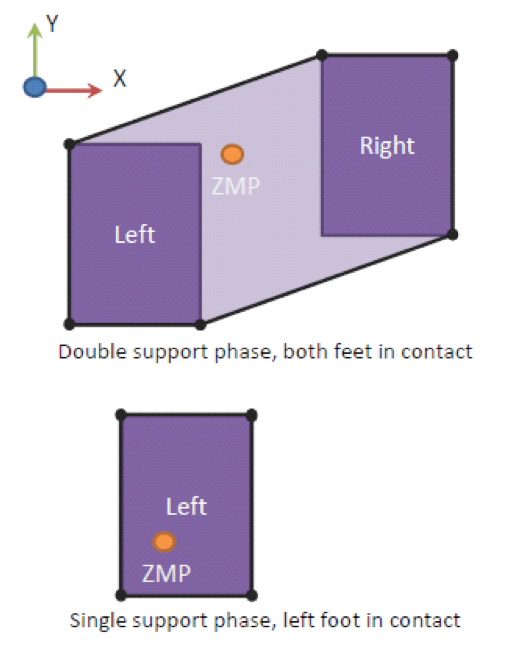
\includegraphics[width=0.5\columnwidth]{./background/pix/zmp.png}
  \caption{Example of the zero moment point on a bipedal robot in a single support phase (bottom) and a double support phase (top).  
If the zero moment point, the location of the center of mass (COM) projected in the direction of gravity, is located within this support polygon then the system is considered statically stable.}
  \label{fig:zmp}
\end{figure}

\noindent \textbf{Single Support Phase}:
The single support phase of a bipedal robot is when a single foot is touching the ground.
This creates a smaller support polygon.

\noindent \textbf{Double Support Phase}:
The double support phase of a bipedal robot is when two feed of a bipedal robot are on the ground.
This creates a larger support polygon.  
In addition there is a stable path that the ZMP can move from above one foot to the other.
This allows the robot to guarantee stability while walking (static walking).

